% Created by tikzDevice version 0.12.6 on 2024-04-16 16:18:13
% !TEX encoding = UTF-8 Unicode
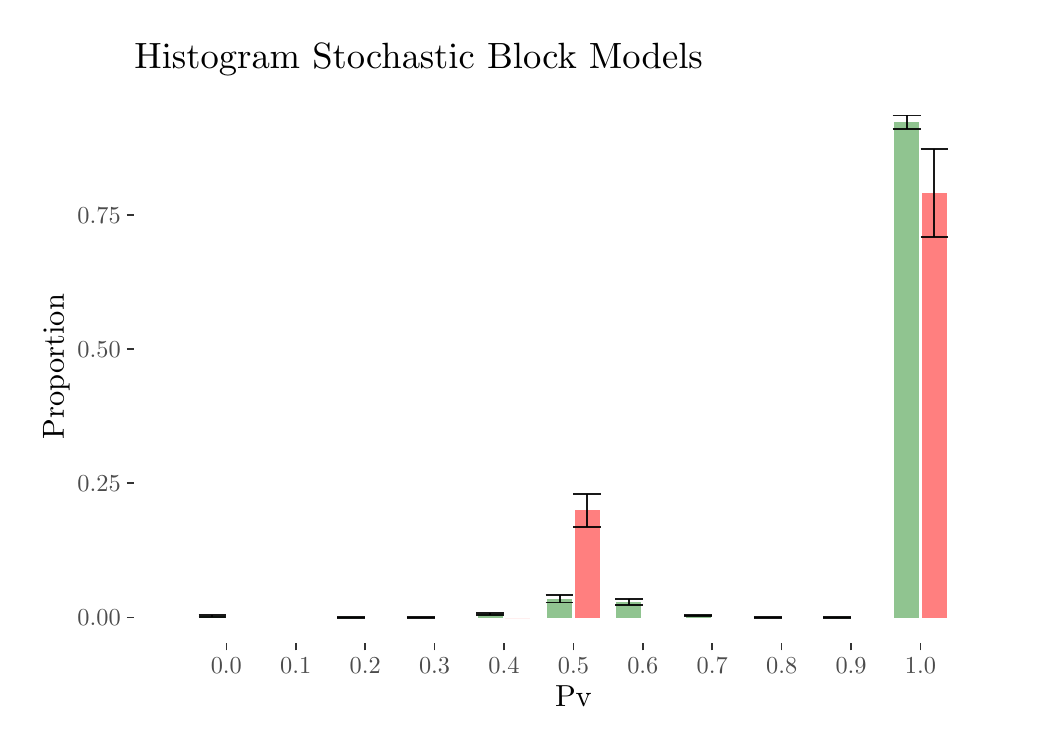
\begin{tikzpicture}[x=1pt,y=1pt]
\definecolor{fillColor}{RGB}{255,255,255}
\path[use as bounding box,fill=fillColor,fill opacity=0.00] (0,0) rectangle (361.35,252.94);
\begin{scope}
\path[clip] (  0.00,  0.00) rectangle (361.35,252.94);
\definecolor{drawColor}{RGB}{255,255,255}
\definecolor{fillColor}{RGB}{255,255,255}

\path[draw=drawColor,line width= 0.6pt,line join=round,line cap=round,fill=fillColor] (  0.00,  0.00) rectangle (361.35,252.94);
\end{scope}
\begin{scope}
\path[clip] ( 38.56, 30.69) rectangle (355.85,230.29);
\definecolor{fillColor}{RGB}{255,255,255}

\path[fill=fillColor] ( 38.56, 30.69) rectangle (355.85,230.29);
\definecolor{fillColor}{RGB}{34,139,34}

\path[fill=fillColor,fill opacity=0.50] ( 62.26, 39.80) rectangle ( 71.29, 40.26);

\path[fill=fillColor,fill opacity=0.50] (112.42, 39.80) rectangle (121.45, 39.80);

\path[fill=fillColor,fill opacity=0.50] (137.51, 39.80) rectangle (146.54, 39.88);

\path[fill=fillColor,fill opacity=0.50] (162.59, 39.80) rectangle (171.62, 41.00);

\path[fill=fillColor,fill opacity=0.50] (187.67, 39.80) rectangle (196.70, 46.62);

\path[fill=fillColor,fill opacity=0.50] (212.75, 39.80) rectangle (221.78, 45.44);

\path[fill=fillColor,fill opacity=0.50] (237.84, 39.80) rectangle (246.87, 40.51);

\path[fill=fillColor,fill opacity=0.50] (262.92, 39.80) rectangle (271.95, 39.85);

\path[fill=fillColor,fill opacity=0.50] (288.00, 39.80) rectangle (297.03, 39.80);

\path[fill=fillColor,fill opacity=0.50] (313.08, 39.80) rectangle (322.11,218.80);
\definecolor{fillColor}{RGB}{255,0,0}

\path[fill=fillColor,fill opacity=0.50] (172.62, 39.80) rectangle (181.65, 39.80);

\path[fill=fillColor,fill opacity=0.50] (197.70, 39.80) rectangle (206.73, 78.57);

\path[fill=fillColor,fill opacity=0.50] (323.12, 39.80) rectangle (332.15,193.12);
\definecolor{drawColor}{RGB}{0,0,0}

\path[draw=drawColor,draw opacity=0.90,line width= 0.7pt,line join=round] ( 61.76, 40.55) --
	( 71.79, 40.55);

\path[draw=drawColor,draw opacity=0.90,line width= 0.7pt,line join=round] ( 66.77, 40.55) --
	( 66.77, 39.97);

\path[draw=drawColor,draw opacity=0.90,line width= 0.7pt,line join=round] ( 61.76, 39.97) --
	( 71.79, 39.97);

\path[draw=drawColor,draw opacity=0.90,line width= 0.7pt,line join=round] (111.92, 39.84) --
	(121.95, 39.84);

\path[draw=drawColor,draw opacity=0.90,line width= 0.7pt,line join=round] (116.94, 39.84) --
	(116.94, 39.77);

\path[draw=drawColor,draw opacity=0.90,line width= 0.7pt,line join=round] (111.92, 39.77) --
	(121.95, 39.77);

\path[draw=drawColor,draw opacity=0.90,line width= 0.7pt,line join=round] (137.00, 40.00) --
	(147.04, 40.00);

\path[draw=drawColor,draw opacity=0.90,line width= 0.7pt,line join=round] (142.02, 40.00) --
	(142.02, 39.77);

\path[draw=drawColor,draw opacity=0.90,line width= 0.7pt,line join=round] (137.00, 39.77) --
	(147.04, 39.77);

\path[draw=drawColor,draw opacity=0.90,line width= 0.7pt,line join=round] (162.09, 41.43) --
	(172.12, 41.43);

\path[draw=drawColor,draw opacity=0.90,line width= 0.7pt,line join=round] (167.10, 41.43) --
	(167.10, 40.57);

\path[draw=drawColor,draw opacity=0.90,line width= 0.7pt,line join=round] (162.09, 40.57) --
	(172.12, 40.57);

\path[draw=drawColor,draw opacity=0.90,line width= 0.7pt,line join=round] (187.17, 48.02) --
	(197.20, 48.02);

\path[draw=drawColor,draw opacity=0.90,line width= 0.7pt,line join=round] (192.19, 48.02) --
	(192.19, 45.22);

\path[draw=drawColor,draw opacity=0.90,line width= 0.7pt,line join=round] (187.17, 45.22) --
	(197.20, 45.22);

\path[draw=drawColor,draw opacity=0.90,line width= 0.7pt,line join=round] (212.25, 46.53) --
	(222.29, 46.53);

\path[draw=drawColor,draw opacity=0.90,line width= 0.7pt,line join=round] (217.27, 46.53) --
	(217.27, 44.36);

\path[draw=drawColor,draw opacity=0.90,line width= 0.7pt,line join=round] (212.25, 44.36) --
	(222.29, 44.36);

\path[draw=drawColor,draw opacity=0.90,line width= 0.7pt,line join=round] (237.33, 40.85) --
	(247.37, 40.85);

\path[draw=drawColor,draw opacity=0.90,line width= 0.7pt,line join=round] (242.35, 40.85) --
	(242.35, 40.18);

\path[draw=drawColor,draw opacity=0.90,line width= 0.7pt,line join=round] (237.33, 40.18) --
	(247.37, 40.18);

\path[draw=drawColor,draw opacity=0.90,line width= 0.7pt,line join=round] (262.42, 39.94) --
	(272.45, 39.94);

\path[draw=drawColor,draw opacity=0.90,line width= 0.7pt,line join=round] (267.43, 39.94) --
	(267.43, 39.76);

\path[draw=drawColor,draw opacity=0.90,line width= 0.7pt,line join=round] (262.42, 39.76) --
	(272.45, 39.76);

\path[draw=drawColor,draw opacity=0.90,line width= 0.7pt,line join=round] (287.50, 39.83) --
	(297.53, 39.83);

\path[draw=drawColor,draw opacity=0.90,line width= 0.7pt,line join=round] (292.52, 39.83) --
	(292.52, 39.77);

\path[draw=drawColor,draw opacity=0.90,line width= 0.7pt,line join=round] (287.50, 39.77) --
	(297.53, 39.77);

\path[draw=drawColor,draw opacity=0.90,line width= 0.7pt,line join=round] (312.58,221.21) --
	(322.62,221.21);

\path[draw=drawColor,draw opacity=0.90,line width= 0.7pt,line join=round] (317.60,221.21) --
	(317.60,216.38);

\path[draw=drawColor,draw opacity=0.90,line width= 0.7pt,line join=round] (312.58,216.38) --
	(322.62,216.38);

\path[draw=drawColor,draw opacity=0.90,line width= 0.7pt,line join=round] (197.20, 84.49) --
	(207.24, 84.49);

\path[draw=drawColor,draw opacity=0.90,line width= 0.7pt,line join=round] (202.22, 84.49) --
	(202.22, 72.64);

\path[draw=drawColor,draw opacity=0.90,line width= 0.7pt,line join=round] (197.20, 72.64) --
	(207.24, 72.64);

\path[draw=drawColor,draw opacity=0.90,line width= 0.7pt,line join=round] (322.62,209.02) --
	(332.65,209.02);

\path[draw=drawColor,draw opacity=0.90,line width= 0.7pt,line join=round] (327.63,209.02) --
	(327.63,177.22);

\path[draw=drawColor,draw opacity=0.90,line width= 0.7pt,line join=round] (322.62,177.22) --
	(332.65,177.22);
\end{scope}
\begin{scope}
\path[clip] (  0.00,  0.00) rectangle (361.35,252.94);
\definecolor{drawColor}{gray}{0.30}

\node[text=drawColor,anchor=base east,inner sep=0pt, outer sep=0pt, scale=  0.88] at ( 33.61, 36.77) {0.00};

\node[text=drawColor,anchor=base east,inner sep=0pt, outer sep=0pt, scale=  0.88] at ( 33.61, 85.27) {0.25};

\node[text=drawColor,anchor=base east,inner sep=0pt, outer sep=0pt, scale=  0.88] at ( 33.61,133.77) {0.50};

\node[text=drawColor,anchor=base east,inner sep=0pt, outer sep=0pt, scale=  0.88] at ( 33.61,182.27) {0.75};
\end{scope}
\begin{scope}
\path[clip] (  0.00,  0.00) rectangle (361.35,252.94);
\definecolor{drawColor}{gray}{0.20}

\path[draw=drawColor,line width= 0.6pt,line join=round] ( 35.81, 39.80) --
	( 38.56, 39.80);

\path[draw=drawColor,line width= 0.6pt,line join=round] ( 35.81, 88.30) --
	( 38.56, 88.30);

\path[draw=drawColor,line width= 0.6pt,line join=round] ( 35.81,136.80) --
	( 38.56,136.80);

\path[draw=drawColor,line width= 0.6pt,line join=round] ( 35.81,185.30) --
	( 38.56,185.30);
\end{scope}
\begin{scope}
\path[clip] (  0.00,  0.00) rectangle (361.35,252.94);
\definecolor{drawColor}{gray}{0.20}

\path[draw=drawColor,line width= 0.6pt,line join=round] ( 71.79, 27.94) --
	( 71.79, 30.69);

\path[draw=drawColor,line width= 0.6pt,line join=round] ( 96.87, 27.94) --
	( 96.87, 30.69);

\path[draw=drawColor,line width= 0.6pt,line join=round] (121.95, 27.94) --
	(121.95, 30.69);

\path[draw=drawColor,line width= 0.6pt,line join=round] (147.04, 27.94) --
	(147.04, 30.69);

\path[draw=drawColor,line width= 0.6pt,line join=round] (172.12, 27.94) --
	(172.12, 30.69);

\path[draw=drawColor,line width= 0.6pt,line join=round] (197.20, 27.94) --
	(197.20, 30.69);

\path[draw=drawColor,line width= 0.6pt,line join=round] (222.29, 27.94) --
	(222.29, 30.69);

\path[draw=drawColor,line width= 0.6pt,line join=round] (247.37, 27.94) --
	(247.37, 30.69);

\path[draw=drawColor,line width= 0.6pt,line join=round] (272.45, 27.94) --
	(272.45, 30.69);

\path[draw=drawColor,line width= 0.6pt,line join=round] (297.53, 27.94) --
	(297.53, 30.69);

\path[draw=drawColor,line width= 0.6pt,line join=round] (322.62, 27.94) --
	(322.62, 30.69);
\end{scope}
\begin{scope}
\path[clip] (  0.00,  0.00) rectangle (361.35,252.94);
\definecolor{drawColor}{gray}{0.30}

\node[text=drawColor,anchor=base,inner sep=0pt, outer sep=0pt, scale=  0.88] at ( 71.79, 19.68) {0.0};

\node[text=drawColor,anchor=base,inner sep=0pt, outer sep=0pt, scale=  0.88] at ( 96.87, 19.68) {0.1};

\node[text=drawColor,anchor=base,inner sep=0pt, outer sep=0pt, scale=  0.88] at (121.95, 19.68) {0.2};

\node[text=drawColor,anchor=base,inner sep=0pt, outer sep=0pt, scale=  0.88] at (147.04, 19.68) {0.3};

\node[text=drawColor,anchor=base,inner sep=0pt, outer sep=0pt, scale=  0.88] at (172.12, 19.68) {0.4};

\node[text=drawColor,anchor=base,inner sep=0pt, outer sep=0pt, scale=  0.88] at (197.20, 19.68) {0.5};

\node[text=drawColor,anchor=base,inner sep=0pt, outer sep=0pt, scale=  0.88] at (222.29, 19.68) {0.6};

\node[text=drawColor,anchor=base,inner sep=0pt, outer sep=0pt, scale=  0.88] at (247.37, 19.68) {0.7};

\node[text=drawColor,anchor=base,inner sep=0pt, outer sep=0pt, scale=  0.88] at (272.45, 19.68) {0.8};

\node[text=drawColor,anchor=base,inner sep=0pt, outer sep=0pt, scale=  0.88] at (297.53, 19.68) {0.9};

\node[text=drawColor,anchor=base,inner sep=0pt, outer sep=0pt, scale=  0.88] at (322.62, 19.68) {1.0};
\end{scope}
\begin{scope}
\path[clip] (  0.00,  0.00) rectangle (361.35,252.94);
\definecolor{drawColor}{RGB}{0,0,0}

\node[text=drawColor,anchor=base,inner sep=0pt, outer sep=0pt, scale=  1.10] at (197.20,  7.64) {Pv};
\end{scope}
\begin{scope}
\path[clip] (  0.00,  0.00) rectangle (361.35,252.94);
\definecolor{drawColor}{RGB}{0,0,0}

\node[text=drawColor,rotate= 90.00,anchor=base,inner sep=0pt, outer sep=0pt, scale=  1.10] at ( 13.08,130.49) {Proportion};
\end{scope}
\begin{scope}
\path[clip] (  0.00,  0.00) rectangle (361.35,252.94);
\definecolor{drawColor}{RGB}{0,0,0}

\node[text=drawColor,anchor=base west,inner sep=0pt, outer sep=0pt, scale=  1.32] at ( 38.56,238.35) {Histogram Stochastic Block Models};
\end{scope}
\end{tikzpicture}
